\documentclass[a4paper,oneside]{Tptesi2}

\usepackage[italian]{babel}
\usepackage{listings}
\usepackage{amsmath,amssymb}
\usepackage{verbatim}
\usepackage{indentfirst}
\usepackage[utf8]{inputenc}
\usepackage{subfigure}
\usepackage{algorithmic}
\usepackage{framed}
\usepackage{rotating}
\usepackage{cite}

% Packages -----------------------------------------------------------------------
%\usepackage{amsthm}
%\usepackage{amsmath}          % Non necessario se usi TPTESI2 perche' gia` incluso
%\usepackage[dvips]{graphicx}  % Non necessario se usi TPTESI2 perche' gia` incluso
%\usepackage{url} %non usare se si usa hyperref


\newcommand{\mr}{\emph{motore di ricerca}}
\newcommand{\Mr}{\emph{Motore di ricerca}}
\newcommand{\ws}{Web~service }


% Use a small font for the verbatim environment
\makeatletter  % makes '@' an ordinary character
\renewcommand{\verbatim@font}{%
  \ttfamily\footnotesize\catcode`\<=\active\catcode`\>=\active%
}
\makeatother   % makes '@' a special symbol again
%
% Simboli Matematici -------------------------------------------------------------
%\newcommand{\h}{\mathcal{H}_\infty} % scorciatoia per sequenza usata spesso
% Definizioni & Teoremi ----------------------------------------------------------
\newtheorem{teorema}{Teorema}[chapter]
\newtheorem{corollario}[teorema]{Corollario}
\newtheorem{lemma}[teorema]{Lemma}
%\theoremstyle{definition}
\newtheorem{definizione}{Definizione}[chapter]
\newtheorem{proposizione}[definizione]{Proposizione}
% Formattazione Figure -----------------------------------------------------------
\setcounter{topnumber}{3}
\setcounter{totalnumber}{3}
\def\topfraction{1}
\def\textfraction{0}
% Fuzz ---------------------------------------------------------------------------
%\hfuzz10cm %Non scassare linee che escono dal bordo
% Frontespizio -------------------------------------------------------------------
       \title{insert title\ldots}
       \author{insert candidate\ldots}
       \titolocorso{Ingegneria Informatica}
       \chair{Prof. ... \\ }
       \numberofmembers{1} %numero dei relatori
       \degreeyear{insert degree year\ldots}
       \numerocorrelatori{2} %numero dei correlatori
       \correlatori{insert correlators\ldots} % i correlatori separati da \\

%
% ---- Inclusioni (vedi piu` sotto per il comando "include" --------------
%\includeonly {introduzione,chapter1, chapter2}
%\includeonly {chapter1, chapter2, chapter3, chapter4, chapter5, chapter6}
%\includeonly{chapter6}
%
\hypersetup{%
%  pdfpagemode=FullScreen,%
  plainpages=false,%
  breaklinks,%
  pdftitle={},%
  pdfauthor={},%
  pdfsubject={},%
  pdfkeywords={},%
  colorlinks=false}

\begin{document}

\frontmatter

%\hyphenation{}
%
\pagestyle{headings} % rende attive le impostazioni sulla testata!
%
\maketitle % crea il frontespizio (ricordati di copiare "stemma.eps" nella tua directory)
%
%
%\pagenumbering{roman}
\tableofcontents % inserisce indice generale
\cleardoublepage
%\addcontentsline{toc}{chapter}{Elenco delle figure}
%\listoffigures   % inserisce indice figure
%\addcontentsline{toc}{chapter}{Elenco delle tabelle}
%\listoftables    % inserisce indice tabelle
%\addcontentsline{toc}{chapter}{Elenco degli algoritmi}
%\listofalgorithms
%
%--------------- Inizio del testo vero e proprio
%

%\cleardoublepage
%\pagenumbering{arabic}
%\input{files/ringraziamenti}
\frontmatter
\chapter{Introduzione}\label{ch:introduzione}
Le intelligente artificiali sono riuscite al giorno d'oggi a risolvere innumerevoli problemi della vita reale come ad esempio il controllo avanzato di alcuni sistemi di automazione, le telecomunicazioni e la robotica. Anche in campo mobile vi sono molti servizi che incorporano IA che sfruttano i dati degli utenti al fine di proporre sistemi altamente personalizzati per le specifiche dell'utente come ad esempio la stessa tastiera qwerty dei nostri dispositivi che è in grado di memorizzare come scriviamo e 'impara' a proporre le prossime parole. Sfruttando le caratteristiche personali dei vari utente  non solo viene migliorata l'esperienza personale ma aiutano anche a controllare meglio i loro dispositivi. \\
La crescente preoccupazione per la privacy dei dati nei vari framework di machine learning esistenti ha alimentato un crescente interesse nello sviluppo di paradigmi di machine learning distribuiti come i framework di apprendimento federato che illustreremo in seguito.


\mainmatter
\chapter{Algoritmo di apprendimento federato}\label{ch:chapter1}
Il Federated Learning è una tecnologia di apprendimento automatico distribuito che permette di addestrare un modello di intelligenza artificiale su un gran numero di apparecchi, mantenendo i dati su ciascun dispositivo.
FL (federated learning) è strutturato in modo che gli agenti di apprendimento si coordinino tramite un server centrale per addestrare un modello di apprendimento distribuito. Questi agenti ricevono il modello di apprendimento locale in base ai set di dati disponibili. Quindi restituiscono i modelli di apprendimento aggiornati al server per l'aggiornamento del modello globale tramite un'operazione di aggregazione senza rivelare i dati di addestramento privato agli altri. In pratica, il set di dati privato raccolto presso ciascun agente è sbilanciato, altamente personalizzato per alcune applicazioni come la scrittura a mano e il riconoscimento vocale e presenta caratteristiche non indipendenti e non identicamente distribuite. Pertanto il processo iterativo di aggiornamento del modello globale migliora la generalizzazione del modello ma danneggia anche le prestazioni personalizzate degli agenti. Quindi gli algoritmi FL esistenti non possono gestire in modo efficiente la relazione coesiva tra la capacità di generalizzazione e personalizzazione del modello di apprendimento addestrato. Vi sono stati alcuni tentativi di studiare e migliorare le prestazioni personalizzate di FL utilizzando un algoritmo di media federata personalizzata (Per-FedAvg) basato su un framework di meta-apprendimento. Si è anche provato ad avere un framework personalizzato adattivo in cui è stata adottata una combinazione di modelli locali e globali per ridurre l'errore di generalizzazione. Tuttavia in entrambi i casi la relazione coesiva tra generalizzazione e personalizzazione non è stata adeguatamente analizzata.\\
In questo elaborato analizzeremo un nuovo framework di apprendimento distribuito che può estendere direttamente lo schema FL convenzionale per risolvere collettivamente un compito di apprendimento comune ai vari agenti. Diversamente dagli algoritmi FL esistenti per la costruzione di un singolo modello generalizzato, manteniamo modelli di gruppo gerarchici autoorganizzanti. Di conseguenza adottiamo il clustering gerarchico agglomerativo e aggiorniamo periodicamente la struttura gerarchica in base alla somiglianza nelle caratteristiche di apprendimento degli utenti. In particolare proponiamo la generalizzazione gerarchica in forma ricorsiva. Per risolvere il complesso problema dato dalla forma ricorsiva, consideriamo  l'algoritmo di apprendimento distribuito: DemLearn. 
% \chapter{Apprendimento democratizzato: concetti}\label{ch:chapter2}
L'algoritmo proposto utilizza lo schema bottom-up per eseguire in modo iterativo l'apprendimento locale risolvendo problemi di apprendimento personalizzati e aggiornando gerarchicamente i modelli generalizzati per gruppi a livelli superiori.\\
Diversamente dall'algoritmo di apprendimento federato, il Dem-AI introduce una struttura gerarchica auto-organizzante per risolvere compiti di apprendimento complessi singoli/multipli mediando i contributi di un gran numero di agenti di apprendimento in un apprendimento collaborativo. Secondo le differenze nelle loro caratteristiche, gli agenti di apprendimento formano gruppi appropriati che possono essere specializzati affinché agenti simili affrontino i compiti di apprendimento. Questi gruppi specializzati sono auto-organizzati in una struttura gerarchica e costruiscono collettivamente la conoscenza di apprendimento generalizzata condivisa per migliorare le loro prestazioni di apprendimento riducendo i problemi individuali dovuti ai dati locali sbilanciati e altamente personalizzati. In particolare, il sistema di apprendimento consente ai nuovi membri del gruppo di accelerare il loro processo di apprendimento con la conoscenza del gruppo esistente e incorporare le loro nuove conoscenze di apprendimento espandendo la capacità di generalizzazione dell'intero gruppo. In questi sistemi ogni agente è libero di unirsi ad uno dei qualsiasi gruppi e possiedono lo stesso potere inteso come numero dei componenti che varierà poi nel tempo.\\
Consideriamo quindi i punti principali del Dem-AI.\\\\
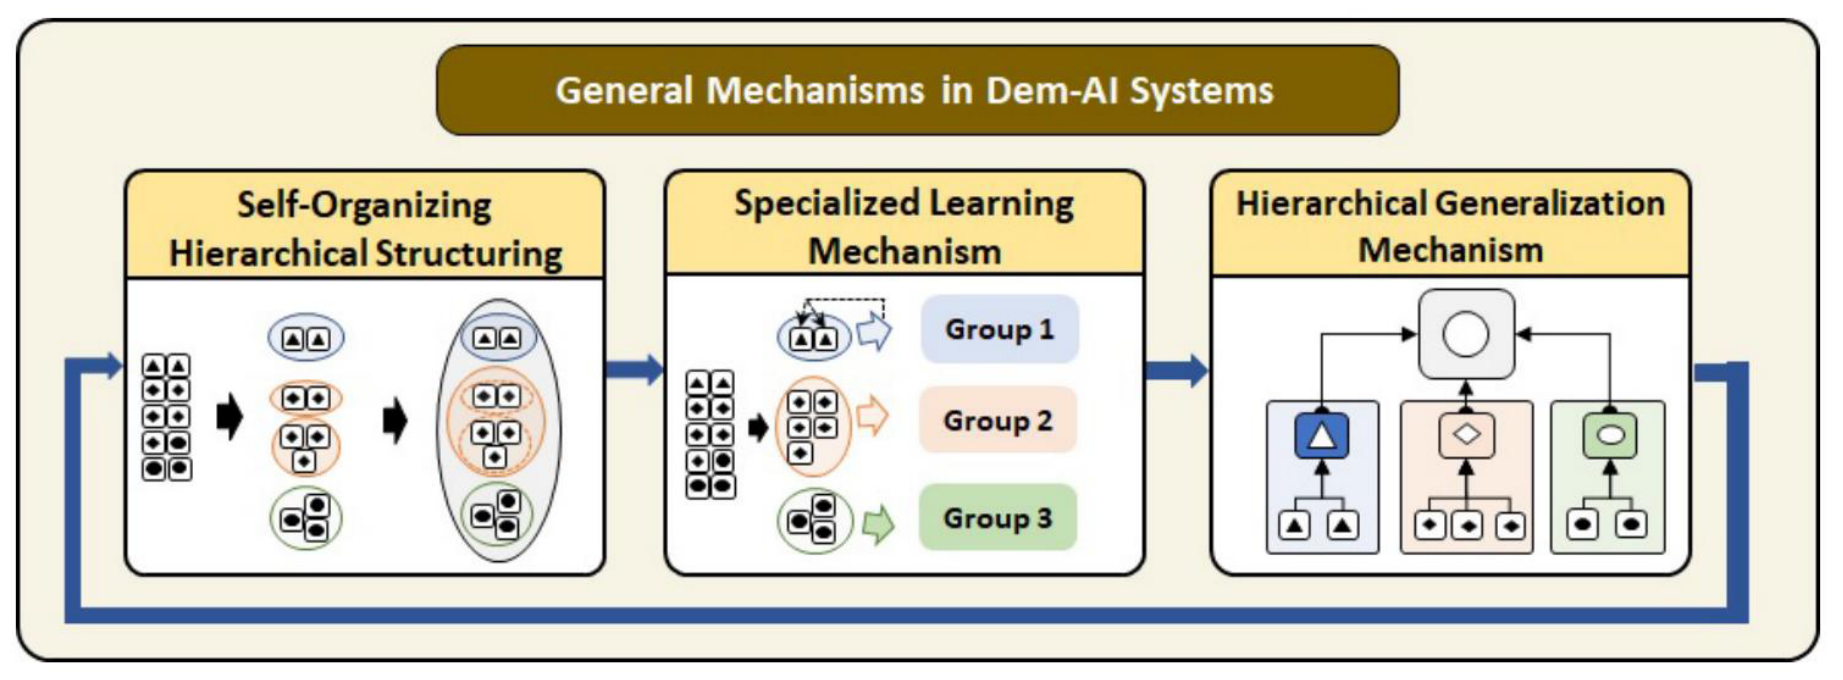
\includegraphics[scale=0.25]{DemIA}

\begin{itemize}

  \item Definizione ed obiettivo\\
  L'apprendimento democratizzato studia processi duali ,accoppiati e operanti insieme, specializzato-generalizzato in una struttura gerarchica auto-organizzante di sistemi di apprendimento distribuiti su larga scala. I processi specializzati e generalizzati devono operare congiuntamente verso un obiettivo di apprendimento finale identificato come l'esecuzione di un apprendimento collettivo da agenti di apprendimento prevenuti, che si impegnano ad apprendere dai propri dati utilizzando le loro limitate capacità di apprendimento. In quanto tale, l'obiettivo finale di apprendimento del sistema Dem-AI è stabilire un meccanismo per risolvere collettivamente compiti di apprendimento complessi comuni (singoli o multipli) da un gran numero di agenti di apprendimento
  \item Processo specializzato\\
  Questo processo viene utilizzato per sfruttare le capacità di apprendimento specializzate degli agenti di apprendimento e dei gruppi specializzati sfruttando i dati raccolti. Incorporando la conoscenza generalizzata dei gruppi di livello superiore creati dal meccanismo di generalizzazione, gli agenti di apprendimento possono aggiornare i parametri del loro modello per ridurre il bias nel loro apprendimento personalizzato.
Pertanto, l'obiettivo di apprendimento personalizzato ha come obiettivi: eseguire un apprendimento specializzato e riutilizzare la conoscenza gerarchica generalizzata disponibile.
  \item Processo generalizzato\\
  Il meccanismo di generalizzazione incoraggia i membri del gruppo a condividere la conoscenza quando svolgono compiti di apprendimento con caratteristiche simili e costruiscono livelli gerarchici di conoscenza generalizzata. La conoscenza gerarchica generalizzata aiuta il sistema Dem-AI a mantenere la capacità di generalizzazione per ridurre il bias degli agenti di apprendimento e affrontare in modo efficiente i cambiamenti ambientali o eseguire nuovi compiti di apprendimento.
  
  \item Struttura gerarchica auto-organizzante\\
  La struttura gerarchica dei gruppi specializzati e le relative conoscenze generalizzate sono costruite e regolate secondo un principio di autoorganizzazione basato sulla somiglianza degli agenti di apprendimento. In particolare, questo principio governa l'unione di piccoli gruppi per formare un gruppo più grande che alla fine migliora le capacità di generalizzazione di tutti i membri. Pertanto, i gruppi specializzati ai livelli più alti nella struttura gerarchica hanno più membri e possono costruire una conoscenza più generalizzata e meno distorta adattandosi più rapidamente ai nuovi ambienti.
  
\item Transizione nel duplice processo specializzato-generalizzato\\
Il processo specializzato diventa sempre più importante rispetto al processo generalizzato durante il periodo di formazione. Di conseguenza, il sistema di apprendimento non solo si evolve per acquisire capacità di specializzazione dai compiti appresi, ma perde anche la capacità di affrontare i cambiamenti ambientali come nuovi agenti di apprendimento e nuovi compiti di apprendimento. Nel frattempo, la struttura gerarchica del sistema Dem-AI è auto-organizzata e si è evoluta da un alto livello di plasticità a un alto livello di stabilità, cioè da gruppi specializzati instabili a gruppi specializzati ben organizzati. La transizione del sistema di apprendimento Dem-AI è illustrata in figura con tre sub-meccanismi iterativi come la generalizzazione, l'apprendimento specializzato e il meccanismo di strutturazione gerarchica. Di conseguenza, la transizione del processo duale specializzato-generalizzato rappresenta le fasi di un tipico quadro di apprendimento democratizzato. In quella transizione, gli agenti di apprendimento sono raggruppati in base alle somiglianze dei loro compiti di apprendimento nella fase iniziale. Quindi, il processo generalizzato aiuta nella costruzione di una conoscenza gerarchica generalizzata per i gruppi specializzati dal basso verso l'alto e incoraggia i membri del gruppo a essere vicini. Nel frattempo, i processi di apprendimento specializzati sfruttano l'apprendimento personalizzato per sfruttare i loro set di dati distorti incorporando la conoscenza di gruppo generalizzata di livello superiore dai gruppi di livello superiore a quelli di livello inferiore.

\end{itemize}

\chapter{Conclusioni}\label{ch:conclusioni}
La nuova filosofia Dem-AI ha fornito linee guida generali per meccanismi di strutturazione gerarchica specializzati, generalizzati e auto-organizzanti in sistemi di machine learning distribuiti su larga scala. Ispirati da queste linee guida, abbiamo formulato i problemi gerarchici di apprendimento generalizzato e sviluppato un nuovo algoritmo di apprendimento distribuito, DemLearn. In questo lavoro, basato sulla somiglianza nelle caratteristiche di apprendimento, il clustering agglomerativo consente l'auto-organizzazione degli agenti di apprendimento in una struttura gerarchica, che viene aggiornata periodicamente. L'analisi dettagliata delle valutazioni sperimentali ha mostrato i vantaggi e gli svantaggi dell'algoritmo proposto. Rispetto al FL convenzionale, mostriamo che DemLearn in modo significativo migliora le prestazioni di generalizzazione dei modelli client senza compromettere in gran parte le prestazioni di specializzazione dei modelli client. Di conseguenza, DemLearn consente buone capacità di apprendimento del compromesso dei modelli client con prestazioni C-SPE e C-GEN elevate, mentre altri algoritmi possono produrre solo modelli locali distorti con capacità generalizzate basse. Queste osservazioni favoriscono una migliore comprensione e un miglioramento delle prestazioni di specializzazione e generalizzazione dei modelli di apprendimento nei futuri sistemi Dem-AI. L'apprendimento democratizzato fornisce ingredienti unici per sviluppare futuri sistemi intelligenti personalizzati distribuiti.
A tal fine, il progetto di apprendimento potrebbe essere ulteriormente studiato con set di dati personalizzati, esteso per capacità di apprendimento multi-task e convalidato con una generalizzazione effettiva per i nuovi utenti e cambiamenti ambientali. Trasformando in realtà i sistemi generali di apprendimento distribuito, il Dem-AI deve essere analizzato in profondità da una varietà di prospettive come la robustezza e la diversità dei modelli di apprendimento e i nuovi meccanismi di trasferimento e distillazione della conoscenza. Inoltre, è possibile incorporare il design flessibile con approcci attuali come meta-learning e metodi basati sull'ottimizzazione per migliorare ulteriormente la personalizzazione in FL.

\addcontentsline{toc}{chapter}{Bibliografia}
\bibliographystyle{plain}
\bibliography{files/biblio}
\bibliographystyle{unsrt}
%\bibliography{sp,xml}

\end{document} 